\frame{\frametitle{Vorbedingungen MediaWiki}
\begin{block}{Webserver}
\begin{itemize}
        \item Wir gehen von einem Apache-Webserver aus, der aus den Repositories gezogen wird.  \pause
        \item \texttt{sudo apt-get install apache2} \pause
\end{itemize}
\end{block}

\begin{block}{PHP}
\begin{itemize}
        \item Wir nutzen die Quellen zur Installation.  \pause
        \item \texttt{sudo apt-get install php5} \pause
\end{itemize}
\end{block}

\begin{block}{MySQL}
\begin{itemize}
        \item Wir nutzen die Quellen zur Installation vom MySQL-Server.  \pause
        \item \texttt{sudo apt-get install mysql-server}
\end{itemize}
\end{block}

}

\frame{\frametitle{Installation MediaWiki Teil I}

\begin{block}{MediaWiki}
\begin{itemize}
        \item Es ist ratsam, jeweils die aktuelleste Version direkt vom Hersteller zu beziehen.  \pause
        \item \texttt{http://www.mediawiki.org/wiki/Download/de} (zurzeit aktuellste Version 1.160 - 12.1 MB schwer) \pause
        \item Der Einfachheit halber nutzern wir ein Unterverzeichnis im Standard-Verzeichnis des Apaches und verzichten auf das Einrichten einer Subdomain. \pause
        \item \texttt{/var/www/wiki} \pause
        \item Dann \texttt{http://servername.tld/wiki} mit dem Browser ansteuern
\end{itemize}
\end{block}

}

\frame{\frametitle{Installation MediaWiki Teil II}

\begin{block}{Site einrichten}
\begin{itemize}
        \item 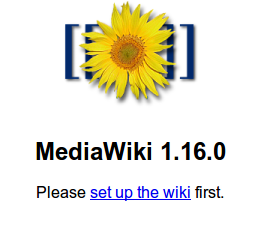
\includegraphics[scale=0.5]{wiki-logo.png} \pause
        \item \pause
        \item \pause

\end{itemize}
\end{block}

}